\documentclass{ieeeaccess}
\usepackage{cite}
\usepackage{amsmath,amssymb,amsfonts}
\usepackage{algorithmic}
\usepackage{graphicx}
\usepackage{textcomp}
\usepackage{hyperref}
\usepackage{booktabs}  % For professional table lines
\usepackage{array}     % For column width handling
\usepackage{bookmark}

\hypersetup{
    colorlinks=true,        % Enable colored links
    linkcolor=blue,         % Internal links (references, sections, etc.)
    citecolor=blue,         % Citation links
    filecolor=blue,         % File links
    urlcolor=blue,          % URL links
    anchorcolor=blue        % Anchor links
}

\usepackage{bm}
\makeatletter
% Fix for missing font shapes in formata font
\DeclareFontShape{T1}{formata}{m}{sl}{<->ssub*formata/m/it}{}
\DeclareFontShape{T1}{formata}{b}{sl}{<->ssub*formata/b/it}{}
\DeclareFontShape{T1}{formata}{bx}{sl}{<->ssub*formata/bx/it}{}

\AtBeginDocument{\DeclareMathVersion{bold}
\SetSymbolFont{operators}{bold}{T1}{times}{b}{n}
\SetSymbolFont{NewLetters}{bold}{T1}{times}{b}{it}
\SetMathAlphabet{\mathrm}{bold}{T1}{times}{b}{n}
\SetMathAlphabet{\mathit}{bold}{T1}{times}{b}{it}
\SetMathAlphabet{\mathbf}{bold}{T1}{times}{b}{n}
\SetMathAlphabet{\mathtt}{bold}{OT1}{pcr}{b}{n}
\SetSymbolFont{symbols}{bold}{OMS}{cmsy}{b}{n}
\renewcommand\boldmath{\@nomath\boldmath\mathversion{bold}}}
\makeatother

\def\BibTeX{{\rm B\kern-.05em{\sc i\kern-.025em b}\kern-.08em
    T\kern-.1667em\lower.7ex\hbox{E}\kern-.125emX}}

%Your document starts from here ___________________________________________________
\begin{document}
\history{Date of publication xxxx 00, 0000, date of current version xxxx 00, 0000.}
\doi{10.1109/ACCESS.2024.0429000}

\title{Generative AI for Analog/RF Integrated Circuit Design and Netlist Synthesis: Evolving Methodologies and Emerging Applications}
\author{\uppercase{Zeyad H. ElSisi}\authorrefmark{1},
\uppercase{Heba M. Draz}\authorrefmark{2}, and Third C. Author,
Jr.\authorrefmark{3},
\IEEEmembership{Member, IEEE}}

\address[1]{National Institute of Standards and
Technology, Boulder, CO 80305 USA (e-mail: author@boulder.nist.gov)}
\address[2]{Department of Physics, Colorado State University, Fort Collins,
CO 80523 USA (e-mail: author@lamar.colostate.edu)}
\address[3]{Electrical Engineering Department, University of Colorado, Boulder, CO
80309 USA}
\tfootnote{This paragraph of the first footnote will contain support
information, including sponsor and financial support acknowledgment. For
example, ``This work was supported in part by the U.S. Department of
Commerce under Grant BS123456.''}

\markboth
{Author \headeretal: Preparation of Papers for IEEE TRANSACTIONS and JOURNALS}
{Author \headeretal: Preparation of Papers for IEEE TRANSACTIONS and JOURNALS}

\corresp{Corresponding author: First A. Author (e-mail: author@ boulder.nist.gov).}


\begin{abstract}
Electronic Design Automation (EDA) in analog Integrated Circuits (ICs) continues to be a critical research area, yet its widespread adoption significantly lags behind its digital counterpart due to inherent complexities. This extended systematic review updates recent contributions in the last five years, specifically highlighting cutting-edge methods that address persistent domain-specific challenges such as data scarcity, efficient topology exploration, robust parameter optimization considering process-voltage-temperature (PVT) variations, and accurate layout parasitic management.
Our primary objective is to equip researchers new to this rapidly evolving domain with a comprehensive collection of references, a refined understanding of current challenges, and practical application guidelines. We provide an in-depth methodological review of state-of-the-art machine learning (ML) and generative AI approaches—including Graph Neural Networks (GNNs), Large Language Models (LLMs), and Variational Autoencoders (VAEs)—which are increasingly applied across various analog circuit design tasks, from topology synthesis to parameter sizing and validation.
Notably, this survey expands on previous works by integrating discussions on newer, comprehensive frameworks like FALCON and MenTeR, which introduce end-to-end design, multi-agent workflows, and advanced layout-aware optimization. To the best of the authors’ knowledge, this is the second review after [1] to comprehensively explore these latest applications of generative AI models in analog IC circuit design, charting their evolution and impact.
We conclude by identifying key future research directions, emphasizing few-shot learning, multi-modal AI, and advanced multi-agent systems to further simplify human-tool interaction and guide design space exploration for industrial-scale analog ICs.
\end{abstract}

\begin{keywords}
Analog integrated circuits (ICs), electronic design automation (EDA), generative artificial intelligence (GenAI), graph neural networks (GNNs), large language models (LLMs), machine learning (ML), netlist synthesis, parameter optimization, layout-aware sizing, topology synthesis, variational autoencoders (VAEs).
\end{keywords}

\titlepgskip=-21pt

\maketitle

\section{Introduction}
\label{sec:introduction}
\PARstart{T}{he} escalating complexity and diverse performance requirements of modern analog systems underpin advancements in crucial technologies such as generative AI, 5G/6G communication, and quantum computing. \textit{"analog genie"}
These demands necessitate full-flow automation to effectively manage the intricate trade-offs between numerous performance parameters, a task where traditional manual approaches are notoriously time-consuming and heavily reliant on scarce expert knowledge. While digital design automation has witnessed extensive development and widespread adoption across both industry and academia, the automation of analog IC design continues to face significant challenges.

Researchers have made concerted efforts to automate various stages of the analog design flow\textit{"genAI paper"}. Conventionally, the process is segmented into three primary areas at the circuit level: topology selection, circuit sizing, and layout generation, often with complex feedback loops, as clearly shown in Fig.~\ref{fig1}.
Although remarkable progress has been achieved in layout generation tools, such as MAGICAL and ALIGN, and in certain aspects of digital IC design with generative AI, the development of scalable and robust solutions for analog circuit sizing and comprehensive topology design remains a formidable challenge. 
Furthermore, a truly practical automation flow at each stage must inherently account for the interdependencies across design stages\textit{"5,6,7 from genAI paper"}; for instance, the initial selection of a topology must proactively consider potential layout parasitics and their subsequent impact on performance metrics.

The fundamental challenge arises from the intricate design complexities of analog ICs. Unlike digital ICs that can be universally and hierarchically abstracted into Boolean logic representations and easily described with high-level hardware description languages (e.g., Verilog and VHDL) or programming languages (e.g., C), analog ICs remain intractable to such abstraction due to their
lack of systematic hierarchical representation and the heuristic and knowledge-intensive nature of their design process~\cite{b1}. This makes automating analog IC design using programming languages similar to those for digital ICs extremely difficult. As such, domain experts have followed a longstanding manual flow to design analog ICs. This process involves a number of time-consuming stages, such as selecting/creating an existing (new) circuit topology (i.e., defining the connections between devices), optimizing device parameters based on the topology to achieve desired performance, and designing the physical layout of the optimized circuit for manufacturing. Importantly, the topology generation stage is the foundation and most creative part of the analog IC design process, posing a formidable and perennial challenge to design automation. Addressing it is the key to accelerating the development of analog ICs.

In response to these challenges, machine learning (ML) has emerged as a promising solution. Learning-based methods, which leverage simulation data for training, offer more efficient design space exploration. 
ML techniques can be applied individually or in combination to facilitate decision-making, function approximation, and black-box optimization. Recent breakthroughs in generative AI, a subset of ML, have presented transformative opportunities to expedite these conventional design flows. 
Models such as Graph Neural Networks (GNNs) have shown significant advantages for handling graph-structured circuit data, while Variational Autoencoders (VAEs) are being explored to learn underlying data distributions for tasks like topology optimization. Furthermore, Large Language Models (LLMs), traditionally used for natural language processing, have demonstrated remarkable adaptability to large-scale design problems, including layout automation, optimization, and topology generation.

Despite these advances, many prior studies on ML-driven analog circuit design have often focused on isolated sub-tasks or simple, homogeneous circuits, overlooking the complexities of real-world heterogeneous systems. \textit{"AI Circuit, }
The persistent lack of comprehensive, generic, and diverse datasets with robust metrics has been a major impediment to thoroughly evaluating and improving ML algorithms in the analog domain. Moreover, many early generative AI approaches for topology generation were limited in scale, producing single types of small or conventional ICs, or suffered from ambiguous representations.
This has encouraged the recent works to try bridging these gaps by proposing more holistic frameworks that integrate multiple design stages, leverage multi-agent systems, and incorporate layout-aware optimization to better reflect practical design scenarios. \textit{"AI Circuit, FALCON, MenTeR "ADO-LLM", "Analog-GENIE", "AMP-AGENT"}

\begin{figure}[h!]
    \centering
    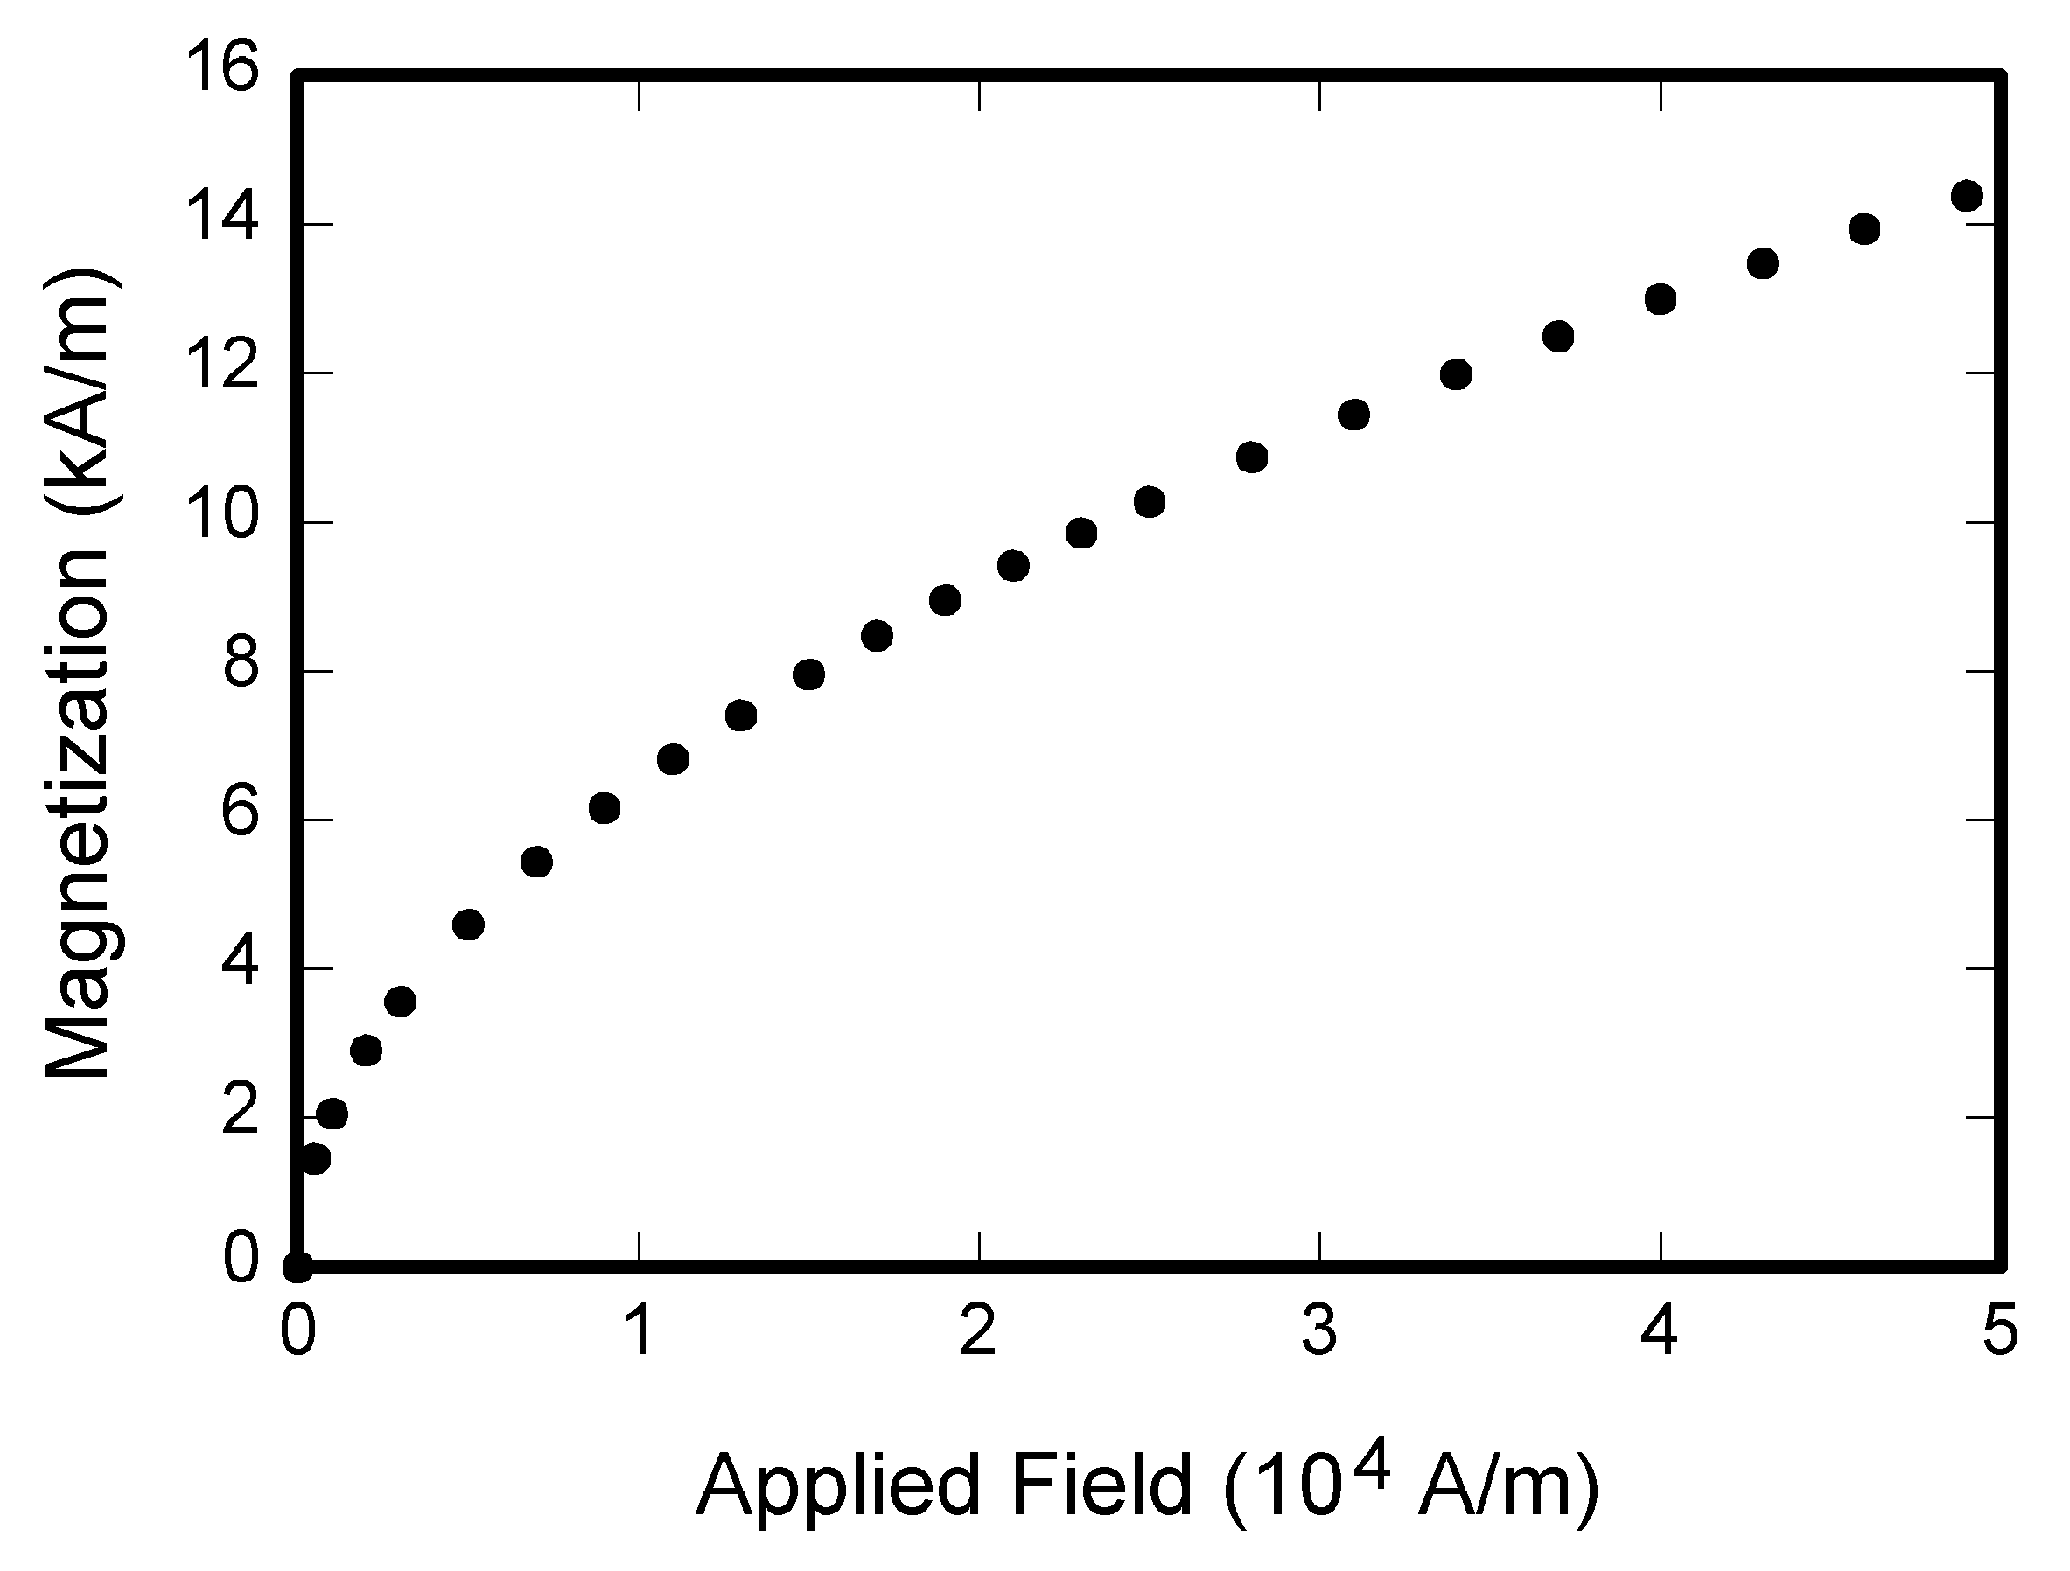
\includegraphics[width=\linewidth]{fig1.png}
    \caption{\textbf{Analog design automation flow, focusing on circuit-level automation. Dashed lines indicate dependencies between design stages.}}
    \label{fig1}
\end{figure}

This paper aims to bridge these gaps by providing an updated and expanded systematic review of generative AI applications in analog IC design. We particularly focus on recent developments that push the boundaries of automation across the entire design pipeline, addressing shortcomings such as data scarcity, limited scalability, and inadequate layout awareness.
Specifically, this review will integrate analysis of groundbreaking new frameworks like:

\begin{itemize}
\item \textbf{AnalogGenie}: A generative engine focused on the automatic discovery of diverse, large, and unseen analog circuit topologies using a scalable sequence-based graph representation and an augmented dataset.
\item \textbf{AnalogCoder}: The first training-free LLM agent that designs analog circuits through Python code generation, employing feedback-enhanced flows and a circuit tool library.
\item \textbf{SPICEPilot}: A framework leveraging LLMs to generate Python-based SPICE code, addressing data scarcity by automating dataset creation and providing standardized benchmarking.
\item \textbf{AnalogXpert}: An LLM-based agent for subcircuit-level SPICE code generation that incorporates circuit design expertise through a proofreading strategy for iterative error correction.
\item \textbf{MenTeR}: A fully-automated multi-agent workflow for end-to-end RF/Analog circuit netlist design, emphasizing specification understanding, collaborative optimization, and test bench validation through Chain-of-Stage reasoning and Diagram-Aware RAG.
\item \textbf{FALCON}: A unified ML framework enabling fully automated, specification-driven analog circuit synthesis through performance-driven topology selection, GNN-based parameter inference, and layout-constrained optimization, validated with industrial-grade simulations.
\item \textbf{AICircuit}: A multi-level dataset and benchmark that facilitates the development and evaluation of ML algorithms for both homogeneous and heterogeneous analog and RF circuit designs.
\item \textbf{AMSNet}: A netlist dataset for Analog and Mixed-Signal (AMS) circuits, which consists of 734 topologies and has been utilized for LLM-based AMS circuit auto-design and netlist generation.
\item \textbf{AnalogCoderPro}: A training-free, end-to-end multimodal LLM framework that unifies topology generation and device sizing. It advances AnalogCoder by incorporating a multimodal diagnosis-and-repair feedback loop that uses simulation logs and waveform images for autonomous error correction.
\end{itemize}

These frameworks represent significant strides toward achieving holistic, human-competitive, and even superhuman capabilities in analog IC design.

The main contributions of this paper are as follows:
\begin{itemize}
\item \textbf{Comprehensive Survey of Recent Advancements}: Examine and compare recent advancements in generative AI for analog circuit design, with a particular focus on evolving techniques that address topology exploration, scalable parameter sizing, robust PVT variations, and realistic layout parasitics.

\item \textbf{Methodological Review of State-of-the-Art Techniques}: Provide a methodological review of state-of-the-art generative AI techniques applied in analog circuit design automation, including Graph Neural Networks (GNNs), Large Language Models (LLMs), and Variational Autoencoders (VAEs), showcasing their latest applications and interconnections.

\item \textbf{Analysis of Novel Comprehensive Frameworks}: Integrate and analyze new, comprehensive frameworks such as FALCON, MenTeR, AnalogGenie, AnalogCoder, SPICEPilot, and AnalogXpert, which were not thoroughly covered in previous surveys, providing insights into their unique contributions and synergistic potential.

\item \textbf{Practical Resource Compilation}: Collect and synthesize abundant resources, open-source codes, and application guidelines to serve as a practical reference for researchers new to or advancing within the field of analog circuit automation.
\end{itemize}
The remainder of this paper is structured as follows: section II summarizes and compares previous review papers in terms of their automation scope and the ML techniques covered, highlighting the gaps addressed by this work. section III introduces fundamental IC design challenges and outlines how these challenges shape the automation task for generative AI. section IV provides the fundamentals of generative AI relevant to recent research, including detailed discussions on GNNs, LLMs, and VAEs. section V comprehensively compares significant research works, focusing on their methodologies, key problems they attempt to solve, and their contributions to the evolving landscape of analog design automation. Finally, section VI outlines future research directions and challenges for large-scale industrial adoption, including discussions on multi-agent systems and multi-modal AI.

%\subsection{Abbreviations and Acronyms}
%Define abbreviations and acronyms the first time they are used in the text,
%even after they have already been defined in the abstract. Abbreviations
%such as IEEE, SI, ac, and dc do not have to be defined. Abbreviations that
%incorporate periods should not have spaces: write ``C.N.R.S.,'' not ``C. N.
%R. S.'' Do not use abbreviations in the title unless they are unavoidable
%(for example, ``IEEE'' in the title of this article).

%\subsection{Other Recommendations}
%Use one space after periods and colons. Hyphenate complex modifiers:
%``zero-field-cooled magnetization.'' Avoid dangling participles, such as,
%``Using \eqref{eq}, the potential was calculated.'' [It is not clear who or what
%used \eqref{eq}.] Write instead, ``The potential was calculated by using \eqref{eq},'' or
%``Using \eqref{eq}, we calculated the potential.''

%Use a zero before decimal points: ``0.25,'' not ``.25.'' Use
%``cm$^{3}$,'' not ``cc.'' Indicate sample dimensions as ``0.1 cm
%$\times $ 0.2 cm,'' not ``0.1 $\times $ 0.2 cm$^{2}$.'' The
%abbreviation for ``seconds'' is ``s,'' not ``sec.'' Use
%``Wb/m$^{2}$'' or ``webers per square meter,'' not
%``webers/m$^{2}$.'' When expressing a range of values, write ``7 to
%9'' or ``7--9,'' not ``7$\sim $9.''

%A parenthetical statement at the end of a sentence is punctuated outside of
%the closing parenthesis (like this). (A parenthetical sentence is punctuated
%within the parentheses.) In American English, periods and commas are within
%quotation marks, like ``this period.'' Other punctuation is ``outside''!
%Avoid contractions; for example, write ``do not'' instead of ``don't.'' The
%serial comma is preferred: ``A, B, and C'' instead of ``A, B and C.''

%If you wish, you may write in the first person singular or plural and use
%the active voice (``I observed that $\ldots$'' or ``We observed that $\ldots$''
%instead of ``It was observed that $\ldots$''). Remember to check spelling. If
%your native language is not English, please get a native English-speaking
%colleague to carefully proofread your paper.

%Try not to use too many typefaces in the same article. Also please remember that MathJax
%can't handle really weird typefaces.



\section{Related Works and Survey Landscape}
The rapid evolution of Artificial Intelligence (AI) and foundation models has spurred numerous systematic reviews aimed at capturing the state-of-the-art in Electronic Design Automation (EDA) "To add all previous survery papers".

This section summarizes the scope of previous survey papers and highlights the critical gaps that this work addresses, particularly concerning the application of generative AI to the complex domain of analog integrated circuits (ICs).


\subsection{Taxonomy of Prior AI for EDA Surveys}
Existing reviews on AI for EDA can generally be categorized into two major types based on the AI paradigm they cover "A survey of circuit foundation models":

\subsubsection{Supervised Predictive AI Techniques}
This category represents the mainstream of earlier AI for EDA solutions "circuit foundation model, generative AI for analog IC", focusing on supervised predictive models tailored for specific tasks, such as early prediction of design quality metrics (e.g., timing, area, power).
These works have been extensively studied and covered in earlier surveys "put all previous surveys". However, they often fall short in addressing the unique challenges of analog IC design, which requires more than just predictive accuracy. The need for creativity in topology generation and the handling of continuous parameter spaces are aspects that these surveys do not fully explore.

\subsubsection{Foundation AI Techniques (Circuit Foundation Models - CFMs)}
This emerging trend focuses on models characterized by pre-training on large datasets followed by fine-tuning for specific applications, enhancing generalization and generative capabilities "put survey of circuit foundation models here".
The concept of Circuit Foundation Models (CFMs) encompasses two primary approaches: encoder-based and decoder-based models. 
Encoder-based models, such as Graph Neural Networks (GNNs), are adept at learning representations from graph-structured data, making them suitable for tasks like topology classification and parameter prediction. 
Decoder-based models, including Variational Autoencoders (VAEs) and Large Language Models (LLMs), excel in generating new designs by learning the underlying distribution of existing circuits.

Most recent surveys on second type CFMs have primarily focused on decoder-based models, specifically Large Language Models (LLMs) for EDA "search of relevant papers in the survey paper". 
This focus reflects the immense generative potential demonstrated by LLMs in areas like Hardware Description Language (HDL) code generation, verification, and debugging "search of relevant papers in the survey paper".

\subsection{Comparison of Coverage and Gaps}

A direct comparison reveals that existing surveys often suffer from limitations in scope, depth of analog coverage, or model inclusivity "pick relevant papers from previous surveys".

\begin{table}[h!]
\caption{\textbf{Comparison of Survey Focus and Gaps}}
\label{tab:survey_comparison}
\setlength{\tabcolsep}{3pt}
\begin{tabular}{|p{35pt}|p{75pt}|p{105pt}|}
\hline
\textbf{Survey} & \textbf{ML/AI Techniques} & \textbf{Gaps Addressed} \\
\hline
\textbf{Traditional Analog Surveys} & 
Bayesian Optimization (BO), \par Evolutionary Algorithms (EA), \par Deep Neural Networks (DNNs), \par Convolutional Neural Networks (CNNs) & 
Lack coverage of generative AI \par (LLMs, VAEs) and end-to-end \par integration; often overlook \par post-layout effects \\
\hline
\textbf{LLM-EDA} & 
Decoder LLMs & 
Lacks encoders (GNNs); \par digital bias; limited \par analog focus \\
\hline
\textbf{Recent Perspectives} & 
Encoder/Decoder LLMs & 
Missing latest GenAI \& \par multi-agent analog \par applications \\
\hline
\end{tabular}
\end{table}

Specific Gaps in Previous Literature:

\subsubsection{Model Inclusivity:} Model inclusivity addresses whether a survey covers the necessary range of AI paradigms critical for analog circuit automation, specifically encompassing both generative and predictive models.
The majority of LLM-focused surveys covered only decoder-based LLMs. This survey, in contrast, incorporates both encoder-based GNNs (used for generalized circuit representation learning and predictive tasks like design quality evaluation) and decoder-based LLMs (used for generative tasks) into a unified CFM framework.

    \begin{itemize}
    \item \textbf{CFM Survey:} (to adjust the link) This work is highly model-inclusive. It systematically defines and categorizes all works within the foundation model paradigm into two primary types: encoder-based methods (which typically learn generalized representations for predictive tasks, e.g., Graph Neural Networks (GNNs)) and decoder-based methods (which leverage Large Language Models (LLMs) for generative tasks). This approach inherently covers the diverse model architectures used across the digital and analog EDA flows.

    \item \textbf{LLM for EDA Survey (The Leak):} The primary limitation of this survey is its exclusive focus on Large Language Models (LLMs), which are decoder-based foundation models. This narrow scope results in a critical omission of foundational encoder-based methods. Many breakthroughs in analog automation rely on non-LLM techniques, such as Graph Neural Networks (GNNs) and Variational Autoencoders (VAEs), which are fundamental for tasks like parasitic modeling and topology generation (e.g., CktGNN). By concentrating solely on LLMs, this survey overlooks a substantial and active segment of foundational analog AI research.

    \item \textbf{Analog AI Survey:} This paper aims to provide a comprehensive methodological review encompassing GNNs, LLMs, and VAEs as applied to analog circuit sizing and automation.
    \end{itemize}

\subsubsection{Analog Depth:} Analog circuit design poses unique challenges, such as complexity due to diverse components, intricate interconnections, and the necessity of direct device-level representation, unlike the high-level abstraction available in digital design.

\begin{itemize}
    \item \textbf{AnalogGenAI Survey}: The AnalogGenAI survey offers the deepest focus, dedicated entirely to analog IC design methodologies and applications. It effectively highlights core analog challenges including data scarcity, topology exploration, PVT variations, and layout parasitics. This survey is particularly rich in techniques for circuit sizing, reinforcement learning, and layout-aware automation. However, much of the research discussed focuses on relatively simple circuits like Op-Amps, with complex systems such as PLLs and power amplifiers being comparatively underexplored.
    \item \textbf{CFM and LLM4EDA Surveys}: Both CFM and LLM4EDA dedicate sections to analog circuits. The CFM survey lists recent works like AnalogGenie, AnalogCoder, and LaMAGIC. The LLM4EDA survey details contributions in initial specification/topology selection, schematic design/simulation (e.g., AnalogCoder, ADO-LLM, LaMAGIC), and layout design (e.g., LLANA, LayoutCopilot).
\end{itemize}

\textbf{Gap and Contribution:} While previous surveys acknowledge the analog domain, detailed coverage of advanced generative capabilities, especially those focusing on scalable and flexible topology discovery, is often summarized. Our survey will emphasize recent breakthroughs that address fundamental analog design difficulties:
\begin{itemize}
\item \textbf{Scalable Topology Discovery}: We highlight approaches like AnalogGenie, which addresses scalable and general analog design by broadening the variety of ICs and increasing device counts. AnalogGenie introduces a sequence-based, pin-level graph representation to efficiently capture large analog circuit topologies, enabling the discovery of diverse and unseen topologies.
\item \textbf{Practical Topology Synthesis}: We examine specialized LLM agents like AnalogXpert, which moves toward practical topology synthesis by formulating it as a subcircuit-level SPICE code generation problem. AnalogXpert achieves significantly higher success rates (40\% on synthetic data, 23\% on real data) compared to baselines like AnalogCoder (8\% and 6\%, respectively) due to its use of a subcircuit library and a human experience-based proofreading strategy.
\end{itemize}

\subsubsection{Emerging Frameworks and Methodologies} Despite the advancements in analog design automation, several challenges remain unaddressed. These include:

    \begin{itemize}
    \item \textbf{End-to-End Automation}: End-to-end automation, spanning from specifications to layout-aware netlists, is identified as a critical future direction across all three existing surveys.
    \newline
    \textbf{Gap and Contribution:} The current literature often tackles topology generation and parameter optimization as separate, sequential stages, which can lead to suboptimal results when inherent topological constraints are ignored during sizing. Our survey highlights new efforts that unify these stages:
    \begin{itemize}
        \item \textbf{Unified Generation and Optimization}: AnalogCoder-Pro is introduced as a training-free, multimodal LLM framework designed for end-to-end analog circuit design, jointly performing topology generation and device sizing. It focuses on transforming natural-language design objectives into optimized netlists.
        \item \textbf{Layout-Constrained Synthesis}: FALCON unifies topology selection, parameter inference, and layout-aware optimization in a single end-to-end pipeline. It guides parameter inference using a differentiable layout cost, integrating schematic and physical considerations.
    \end{itemize}
    \item \textbf{Multi-Agent and Feedback Systems}: The use of autonomous agents and sophisticated feedback loops is crucial for handling the complexity and iterative nature of analog design.
    \newline
    The LLM4EDA survey notes the trend toward LLM autonomous agents that iteratively improve code quality by incorporating feedback. It specifically mentions LayoutCopilot as an LLM-powered multi-agent collaborative framework for analog layout design. AnalogCoder employs a feedback-enhanced design flow to refine generated circuits based on functional checks and simulation results.
    \newline
    \textbf{Gap and Contribution:} Recent advancements incorporate multi-modal inputs and highly specialized agents to improve robustness and efficiency beyond basic feedback loops:
        \begin{itemize}
        \item \textbf{Multi-Modal Diagnosis:}:AnalogCoder-Pro advances the feedback loop by incorporating a multimodal diagnosis-and-repair feedback loop that utilizes simulation error messages and waveform images to autonomously correct design errors.
        \item \textbf{Specialized Multi-Agent Systems:} MenTeR proposes a fully-automated multi-agent workflow integrated into an end-to-end analog design framework. It uses specialized agents for specification understanding, design refinement via Chain-of-Stage (CoS) reasoning, and diagram-aware retrieval, demonstrating significant performance improvements over single-agent approaches, even tackling complex circuits like the CMOS Bandgap Reference. Similarly, AmpAgent is an LLM-based multi-agent system specifically for multi-stage amplifier schematic design.
    \end{itemize}
    \item \textbf{Data Scarcity Solutions}: The lack of large, high-quality, and publicly available analog circuit datasets remains a fundamental bottleneck.
    \newline
    All three existing surveys recognize this challenge. The CFM survey explicitly discusses synthetic dataset generation and advanced data augmentation techniques as necessary paths forward. The AnalogGenAI survey advocates for the creation of open-source datasets and testbenches like AICircuit.
    \newline
    \textbf{Gap and Contribution:} Our survey highlights critical recent efforts focused on generating large-scale, automated, and multi-modal analog datasets, which are essential for training robust foundation models.
    \begin{itemize}
        \item \textbf{Generative Dataset Creation:} We discuss new automated frameworks designed to extract data at scale. AnalogGenie addressed this gap by building an extensive dataset of over 3,000 distinct analog circuit topologies with diverse functionalities, expanded by over 70x using data augmentation.
        \item \textbf{Automated Schematic-to-Netlist Extraction:} We review frameworks dedicated to overcoming the image-to-netlist conversion barrier. Masala-CHAI is a fully automated framework leveraging LLMs and custom deep network models to generate SPICE netlists from schematic images, resulting in the largest curated open-source dataset of $\sim$7,500 SPICE netlists from textbooks. Similarly, AMSnet 2.0 uses deep-learning-based image instance segmentation for robust net detection to generate netlists and subsequently reconstruct digital schematics, overcoming the limitations of previous heuristic methods on noisy schematics. These tools directly address the deficiency of SPICE netlist data compared to digital HDL code and don't need to forget SPICE\-Pilot; which is based on LLM-generated SPICE datasets.
    \end{itemize}
    \end{itemize}

By focusing on these specific advancements—particularly the deep integration of multi-modal data, multi-agent reasoning, unified topology-sizing optimization, and large-scale dataset generation—our survey provides a current and comprehensive understanding of the Generative AI landscape for complex analog circuit design, building upon and extending the scope of the existing literature.

By incorporating over 130 relevant works, spanning both predictive (encoder-based) and generative (decoder-based) methodologies, this survey provides a comprehensive collection of resources and application guidelines for researchers targeting industrial-scale analog IC design challenges.

\section{Fundamental Analog IC Design Challenges}

The quest for automating Analog Integrated Circuit (IC) design is obstructed by several foundational challenges inherent to continuous-signal processing, which contrast sharply with the structured nature of digital design. These challenges drive the complexity of the design cycle and necessitate advanced generative AI solutions.

\subsection{Design Stages: Topology Selection, Circuit Sizing, and Layout Generation}
The conventional manual flow segments the design into three critical, tightly coupled stages: topology selection, circuit sizing (parameter inference), and layout generation. A persistent challenge is the inherent strong interdependency across these stages. The performance of a circuit hinges on the topological choices, parameter values, and eventual physical implementation, where optimization in one stage often restricts success in the next.

\begin{enumerate}
    \item \textbf{Topology Selection and Synthesis:} This is widely regarded as the most creative and challenging initial phase. Automation efforts must overcome the immense design space and the lack of a universal, scalable representation method for circuits. Frameworks like AnalogGenie address this by proposing models that can automatically discover diverse, large, and previously unseen circuit topologies.
    
    \item \textbf{Circuit Sizing and Parameter Optimization:} This stage involves setting precise physical dimensions (W/L ratios, component values) to meet specific performance targets. As the number of parameters increases, optimization becomes computationally intensive and prone to local minima.
    
    \item \textbf{Layout Generation:} The final stage demands adherence to complex manufacturing constraints while mitigating physical effects.
\end{enumerate}

\subsection{Intricate Trade-offs and Non-Linearity}
Analog circuits must successfully navigate numerous, often contradictory, performance requirements simultaneously, such as Power, Performance, Area (PPA), in addition to noise, gain, and linearity.

\begin{enumerate}
    \item \textbf{Conflicting Metrics and Application Specificity:} Improving one metric often degrades another (e.g., increasing device size improves noise performance but increases parasitics and reduces speed). Moreover, analog IC design is highly application-specific, relying on designer intuition to define context-dependent Figures of Merit (FoM) and acceptable compromises.
    
    \item \textbf{High Non-Linearity:} The relationship between circuit parameters and performance metrics is often highly non-linear, especially in complex circuits. AICircuit highlights this issue, noting that metrics such as phase noise in Voltage-Controlled Oscillators (VCOs) and performance metrics in Power Amplifiers (PAs) are difficult for even advanced models (MLPs, Transformers) to learn effectively.
\end{enumerate}

\subsection{Abstraction Gap and Design Complexity}
Analog circuits exhibit a fundamental complexity rooted in the continuous nature of signals and their low-level representation:

\begin{enumerate}
    \item \textbf{Low-Level Representation:} Unlike digital circuits, which can be abstracted hierarchically into Boolean logic using high-level Hardware Description Languages (HDLs), analog circuits resist such simplification. Analog design inherently operates at the device level. Even basic functions, such as an analog adder, require explicit configuration and wiring of multiple MOSFETs and resistors, unlike a succinct digital implementation.
    
    \item \textbf{Combinatorial Complexity:} Analog circuits comprise a diverse mixture of voltage sources, MOSFETs, resistors, and capacitors. The intricate interconnections mean that even minor parameter adjustments can drastically alter functionality, potentially leading to a combinatorial explosion in the design search space.
    
    \item \textbf{Heterogeneous Systems:} Scaling solutions to real-world, complex heterogeneous circuits (systems combining blocks with distinct functionalities, like a transmitter combining a VCO and a PA) remains challenging. Critically, AICircuit demonstrated that models trained on individual homogeneous circuits cannot generalize well to large heterogeneous systems due to load effects and strong coupling between blocks.
\end{enumerate}

\subsection{Data Scarcity and Acquisition Bottleneck}
The scarcity of large, comprehensive analog circuit datasets is a severe barrier to applying generative AI methods.

\begin{enumerate}
    \item \textbf{Proprietary Data and Language Scarcity:} Semiconductor companies protect proprietary designs, leading to few publicly available datasets. Furthermore, SPICE (Simulation Program with Integrated Circuit Emphasis), the predominant language for analog netlists, has a much smaller footprint in public code repositories compared to digital HDLs (like Verilog), complicating LLM domain learning.

    \item \textbf{Schema-to-Netlist Bottleneck:} Much of the available analog design information exists only as schematic diagrams in papers and textbooks. Converting these schematic images into executable SPICE netlists typically requires painstaking manual transcription.

    \item \textbf{Addressing Data Needs:}

    \begin{itemize}
        \item \textbf{AMSnet 2.0}: Directly tackles this data bottleneck by constructing a large-scale database comprising transistor-level schematics, SPICE netlists, and component positional information. This resource is crucial for training Multimodal Large Language Models (MLLMs) to recognize and understand schematics.
        \item \textbf{AICircuit}: Provides a comprehensive, high-fidelity, multi-level benchmark dataset covering both homogeneous and complex heterogeneous circuits simulated using commercial tools.
        \item \textbf{AnalogGenie}: Addressed data scarcity by collecting an extensive dataset of over 3,000 diverse circuit topologies and employing data augmentation techniques to expand it substantially.
        \item \textbf{Frameworks like AnalogCoder and SPICEPilot}: Utilize LLMs to generate functional Python/PySpice code, effectively generating synthetic data and accelerating dataset creation.
    \end{itemize}
\end{enumerate}

\subsection{PVT Variations and Robustness}
Analog designs must be robust against Process, Voltage, and Temperature (PVT) variations. A design optimized under nominal conditions may fail under worst-case scenarios, necessitating computationally expensive PVT corner analysis to ensure design viability.

\subsection{Layout Parasitics and Physical Awareness}
The transition from schematic-level design to physical layout introduces parasitic effects that critically influence performance, especially in high-frequency (RF/mm-wave) and advanced technology nodes. Ignoring these effects leads to schematic-to-layout mismatch.

\begin{enumerate}
    \item \textbf{Unified Layout Constraints:} The FALCON framework unifies the schematic and physical domain by incorporating layout constraints directly into the optimization loop. It uses a differentiable layout model to analytically compute area penalties and enforce design rules during gradient-based parameter inference, guiding the optimization toward physically realizable solutions.

    \item \textbf{Multimodal Diagnosis:} AnalogCoder-Pro addresses the challenge of layout-sensitive performance by integrating a multimodal diagnosis-and-repair feedback loop. This system can analyze complex non-textual data, such as waveforms and frequency response images, to diagnose issues related to physical effects that textual logs might miss, improving the design refinement process.
\end{enumerate}

\subsection{Ambiguity, Heuristics, and the Need for Unified Flows}
The reliance on expert intuition and heuristic decision-making in analog design makes formalizing the design process for AI challenging.

\begin{enumerate}
    \item \textbf{Topology-Sizing Decoupling:} Traditionally, topology generation and device sizing are treated sequentially, often resulting in suboptimal choices that lead to expensive, iterative redesigns.
    \item \textbf{Unified and Agentic Approaches:} Generative AI aims to capture and operationalize this expertise:
        \begin{itemize}
            \item \textbf{AnalogCoder-Pro:} addresses the decoupling challenge by aiming for a unified framework that combines topology generation and device sizing, supported by multimodal feedback and a circuit tool library for managing component reuse.
            \item \textbf{AnalogCoder:} introduced a training-free LLM agent utilizing a prompt engineering and a feedback-enhanced flow to achieve automated design and self-correction.
            \item \textbf{AnalogXpert:} focuses on incorporating human expertise by formulating topology synthesis as a subcircuit-level task complemented by a proofreading strategy that allows the LLM agent to iteratively correct errors based on predefined design rules.
            \item \textbf{MenTeR:} uses a multi-agent framework powered by Chain-of-Stage (CoS) reasoning to decompose complex problems and employs Diagram-Aware RAG (DA-RAG) to retrieve information, ensuring that expert knowledge embedded in diagrams is effectively used throughout the design flow.
        \end{itemize}
\end{enumerate}

Please don't use the \verb|{eqnarray}| equation environment. Use
\verb|{align}| or \verb|{IEEEeqnarray}| instead. The \verb|{eqnarray}|
environment leaves unsightly spaces around relation symbols.

Please note that the \verb|{subequations}| environment in {\LaTeX}
will increment the main equation counter even when there are no
equation numbers displayed. If you forget that, you might write an
article in which the equation numbers skip from (17) to (20), causing
the copy editors to wonder if you've discovered a new method of
counting.

{\BibTeX} does not work by magic. It doesn't get the bibliographic
data from thin air but from .bib files. If you use {\BibTeX} to produce a
bibliography you must send the .bib files.

{\LaTeX} can't read your mind. If you assign the same label to a
subsubsection and a table, you might find that Table I has been cross
referenced as Table IV-B3.

{\LaTeX} does not have precognitive abilities. If you put a
\verb|\label| command before the command that updates the counter it's
supposed to be using, the label will pick up the last counter to be
cross referenced instead. In particular, a \verb|\label| command
should not go before the caption of a figure or a table.

Do not use \verb|\nonumber| inside the \verb|{array}| environment. It
will not stop equation numbers inside \verb|{array}| (there won't be
any anyway) and it might stop a wanted equation number in the
surrounding equation.


\Figure[t!](topskip=0pt, botskip=0pt, midskip=0pt){fig2.png}
{ \textbf{Magnetization as a function of applied field.
It is good practice to explain the significance of the figure in the caption.}\label{fig2}}

\section{Some Common Mistakes}
The word ``data'' is plural, not singular. The subscript for the
permeability of vacuum $\mu _{0}$ is zero, not a lowercase letter
``o.'' The term for residual magnetization is ``remanence''; the adjective
is ``remanent''; do not write ``remnance'' or ``remnant.'' Use the word
``micrometer'' instead of ``micron.'' A graph within a graph is an
``inset,'' not an ``insert.'' The word ``alternatively'' is preferred to the
word ``alternately'' (unless you really mean something that alternates). Use
the word ``whereas'' instead of ``while'' (unless you are referring to
simultaneous events). Do not use the word ``essentially'' to mean
``approximately'' or ``effectively.'' Do not use the word ``issue'' as a
euphemism for ``problem.'' When compositions are not specified, separate
chemical symbols by en-dashes; for example, ``NiMn'' indicates the
intermetallic compound Ni$_{0.5}$Mn$_{0.5}$ whereas
``Ni--Mn'' indicates an alloy of some composition
Ni$_{x}$Mn$_{1-x}$.

Be aware of the different meanings of the homophones ``affect'' (usually a
verb) and ``effect'' (usually a noun), ``complement'' and ``compliment,''
``discreet'' and ``discrete,'' ``principal'' (e.g., ``principal
investigator'') and ``principle'' (e.g., ``principle of measurement''). Do
not confuse ``imply'' and ``infer.''

Prefixes such as ``non,'' ``sub,'' ``micro,'' ``multi,'' and ``ultra'' are
not independent words; they should be joined to the words they modify,
usually without a hyphen. There is no period after the ``et'' in the Latin
abbreviation ``\emph{et al.}'' (it is also italicized). The abbreviation ``i.e.,'' means
``that is,'' and the abbreviation ``e.g.,'' means ``for example'' (these
abbreviations are not italicized).

A general IEEE styleguide is available at \break
\underline{http://www.ieee.org/authortools}.

\section{Guidelines for Graphics Preparation and Submission}
\label{sec:guidelines}

\subsection{Types of Graphics}
The following list outlines the different types of graphics published in
IEEE journals. They are categorized based on their construction, and use of
color/shades of gray:

\subsubsection{Color/Grayscale figures}
{Figures that are meant to appear in color, or shades of black/gray. Such
figures may include photographs, illustrations, multicolor graphs, and
flowcharts. For multicolor graphs, please avoid any gray backgrounds or shading, as well as screenshots, instead export the graph from the program used to collect the data.}

\subsubsection{Line Art figures}
{Figures that are composed of only black lines and shapes. These figures
should have no shades or half-tones of gray, only black and white.}

\subsubsection{Author photos}
{Author photographs should be included with the author biographies located at the end of the article underneath References. }

\subsubsection{Tables}
{Data charts which are typically black and white, but sometimes include
color.}

\begin{table}
\caption{\textbf{Units for Magnetic Properties}}
\label{table}
\setlength{\tabcolsep}{3pt}
\begin{tabular}{|p{25pt}|p{75pt}|p{115pt}|}
\hline
Symbol&
Quantity&
Conversion from Gaussian and \par CGS EMU to SI $^{\mathrm{a}}$ \\
\hline
$\Phi $&
magnetic flux&
1 Mx $\to  10^{-8}$ Wb $= 10^{-8}$ V$\cdot $s \\
$B$&
magnetic flux density, \par magnetic induction&
1 G $\to  10^{-4}$ T $= 10^{-4}$ Wb/m$^{2}$ \\
$H$&
magnetic field strength&
1 Oe $\to  10^{3}/(4\pi )$ A/m \\
$m$&
magnetic moment&
1 erg/G $=$ 1 emu \par $\to 10^{-3}$ A$\cdot $m$^{2} = 10^{-3}$ J/T \\
$M$&
magnetization&
1 erg/(G$\cdot $cm$^{3}) =$ 1 emu/cm$^{3}$ \par $\to 10^{3}$ A/m \\
4$\pi M$&
magnetization&
1 G $\to  10^{3}/(4\pi )$ A/m \\
$\sigma $&
specific magnetization&
1 erg/(G$\cdot $g) $=$ 1 emu/g $\to $ 1 A$\cdot $m$^{2}$/kg \\
$j$&
magnetic dipole \par moment&
1 erg/G $=$ 1 emu \par $\to 4\pi \times  10^{-10}$ Wb$\cdot $m \\
$J$&
magnetic polarization&
1 erg/(G$\cdot $cm$^{3}) =$ 1 emu/cm$^{3}$ \par $\to 4\pi \times  10^{-4}$ T \\
$\chi , \kappa $&
susceptibility&
1 $\to  4\pi $ \\
$\chi_{\rho }$&
mass susceptibility&
1 cm$^{3}$/g $\to  4\pi \times  10^{-3}$ m$^{3}$/kg \\
$\mu $&
permeability&
1 $\to  4\pi \times  10^{-7}$ H/m \par $= 4\pi \times  10^{-7}$ Wb/(A$\cdot $m) \\
$\mu_{r}$&
relative permeability&
$\mu \to \mu_{r}$ \\
$w, W$&
energy density&
1 erg/cm$^{3} \to  10^{-1}$ J/m$^{3}$ \\
$N, D$&
demagnetizing factor&
1 $\to  1/(4\pi )$ \\
\hline
\multicolumn{3}{p{251pt}}{Vertical lines are optional in tables. Statements that serve as captions for
the entire table do not need footnote letters. }\\
\multicolumn{3}{p{251pt}}{$^{\mathrm{a}}$Gaussian units are the same as cg emu for magnetostatics; Mx
$=$ maxwell, G $=$ gauss, Oe $=$ oersted; Wb $=$ weber, V $=$ volt, s $=$
second, T $=$ tesla, m $=$ meter, A $=$ ampere, J $=$ joule, kg $=$
kilogram, H $=$ henry.}
\end{tabular}
\label{tab1}
\end{table}

\subsection{Multipart figures}
Figures compiled of more than one sub-figure presented side-by-side, or
stacked. If a multipart figure is made up of multiple figure
types (one part is lineart, and another is grayscale or color) the figure
should meet the stricter guidelines.

\subsection{File Formats For Graphics}\label{formats}
Format and save your graphics using a suitable graphics processing program
that will allow you to create the images as PostScript (.PS), Encapsulated
PostScript (.EPS), Tagged Image File Format (.TIFF), Portable Document
Format (.PDF), Portable Network Graphics (.PNG), or Metapost (.MPS), sizes them, and adjusts
the resolution settings. When
submitting your final paper, your graphics should all be submitted
individually in one of these formats along with the manuscript.

\subsection{Sizing of Graphics}
Most charts, graphs, and tables are one column wide (3.5 inches/88
millimeters/21 picas) or page wide (7.16 inches/181 millimeters/43
picas). The maximum depth a graphic can be is 8.5 inches (216 millimeters/54
picas). When choosing the depth of a graphic, please allow space for a
caption. Figures can be sized between column and page widths if the author
chooses, however it is recommended that figures are not sized less than
column width unless when necessary.

There is currently one publication with column measurements that do not
coincide with those listed above. Proceedings of the IEEE has a column
measurement of 3.25 inches (82.5 millimeters/19.5 picas).

The final printed size of author photographs is exactly
1 inch wide by 1.25 inches tall (25.4 millimeters$\,\times\,$31.75 millimeters/6
picas$\,\times\,$7.5 picas). Author photos printed in editorials measure 1.59 inches
wide by 2 inches tall (40 millimeters$\,\times\,$50 millimeters/9.5 picas$\,\times\,$12
picas).

\subsection{Resolution }
The proper resolution of your figures will depend on the type of figure it
is as defined in the ``Types of Figures'' section. Author photographs,
color, and grayscale figures should be at least 300dpi. Line art, including
tables should be a minimum of 600dpi.

\subsection{Vector Art}
In order to preserve the figures' integrity across multiple computer
platforms, we accept files in the following formats: .EPS/.PDF/.PS. All
fonts must be embedded or text converted to outlines in order to achieve the
best-quality results.

\subsection{Color Space}
The term color space refers to the entire sum of colors that can be
represented within the said medium. For our purposes, the three main color
spaces are Grayscale, RGB (red/green/blue) and CMYK
(cyan/magenta/yellow/black). RGB is generally used with on-screen graphics,
whereas CMYK is used for printing purposes.

All color figures should be generated in RGB or CMYK color space. Grayscale
images should be submitted in Grayscale color space. Line art may be
provided in grayscale OR bitmap colorspace. Note that ``bitmap colorspace''
and ``bitmap file format'' are not the same thing. When bitmap color space
is selected, .TIF/.TIFF/.PNG are the recommended file formats.

\subsection{Accepted Fonts Within Figures}
When preparing your graphics IEEE suggests that you use of one of the
following Open Type fonts: Times New Roman, Helvetica, Arial, Cambria, and
Symbol. If you are supplying EPS, PS, or PDF files all fonts must be
embedded. Some fonts may only be native to your operating system; without
the fonts embedded, parts of the graphic may be distorted or missing.

A safe option when finalizing your figures is to strip out the fonts before
you save the files, creating ``outline'' type. This converts fonts to
artwork what will appear uniformly on any screen.

\subsection{Using Labels Within Figures}

\subsubsection{Figure Axis labels }
Figure axis labels are often a source of confusion. Use words rather than
symbols. As an example, write the quantity ``Magnetization,'' or
``Magnetization M,'' not just ``M.'' Put units in parentheses. Do not label
axes only with units. As in Fig. 1, for example, write ``Magnetization
(A/m)'' or ``Magnetization (A$\cdot$m$^{-1}$),'' not just ``A/m.'' Do not label axes with a ratio of quantities and
units. For example, write ``Temperature (K),'' not ``Temperature/K.''

Multipliers can be especially confusing. Write ``Magnetization (kA/m)'' or
``Magnetization (10$^{3}$ A/m).'' Do not write ``Magnetization
(A/m)$\,\times\,$1000'' because the reader would not know whether the top
axis label in Fig. 1 meant 16000 A/m or 0.016 A/m. Figure labels should be
legible, approximately 8 to 10 point type.

\subsubsection{Subfigure Labels in Multipart Figures and Tables}
Multipart figures should be combined and labeled before final submission.
Labels should appear centered below each subfigure in 8 point Times New
Roman font in the format of (a) (b) (c).

\subsection{File Naming}
Figures (line artwork or photographs) should be named starting with the
first 5 letters of the author's last name. The next characters in the
filename should be the number that represents the sequential
location of this image in your article. For example, in author
``Anderson's'' paper, the first three figures would be named ander1.tif,
ander2.tif, and ander3.ps.

Tables should contain only the body of the table (not the caption) and
should be named similarly to figures, except that `.t' is inserted
in-between the author's name and the table number. For example, author
Anderson's first three tables would be named ander.t1.tif, ander.t2.ps,
ander.t3.eps.

Author photographs should be named using the first five characters of the
pictured author's last name. For example, four author photographs for a
paper may be named: oppen.ps, moshc.tif, chen.eps, and duran.pdf.

If two authors or more have the same last name, their first initial(s) can
be substituted for the fifth, fourth, third$\ldots$ letters of their surname
until the degree where there is differentiation. For example, two authors
Michael and Monica Oppenheimer's photos would be named oppmi.tif, and
oppmo.eps.

\subsection{Referencing a Figure or Table Within Your Paper}
When referencing your figures and tables within your paper, use the
abbreviation ``Fig.'' even at the beginning of a sentence. Figures should be numbered with Arabic Numerals.
Do not abbreviate ``Table.'' Tables should be numbered with Roman Numerals.

\subsection{Submitting Your Graphics}
Figures should be submitted individually, separate from the manuscript in one of the file formats listed above in Section IV-C. Place figure captions below the figures; place table titles above the tables. Please do not include captions as part of the figures, or put them in ‘‘text boxes’’ linked to the figures. Also, do not place borders around the outside of your figures.

\subsection{Color Processing/Printing in IEEE Journals}
All IEEE Transactions, Journals, and Letters allow an author to publish
color figures on IEEE {\it Xplore}$\circledR$\ at no charge, and automatically
convert them to grayscale for print versions. In most journals, figures and
tables may alternatively be printed in color if an author chooses to do so.
Please note that this service comes at an extra expense to the author. If
you intend to have print color graphics, include a note with your final
paper indicating which figures or tables you would like to be handled that
way, and stating that you are willing to pay the additional fee.

\section{Conclusion}
Although a conclusion may review the  main points of the paper, do not replicate the abstract as the conclusion. A
conclusion might elaborate on the importance of the work or suggest
applications and extensions.

If you have multiple appendices, use the $\backslash$appendices command below. If you have only one appendix, use
$\backslash$appendix[Appendix Title]

\appendices
\section{\break Footnotes}
Number footnotes separately in superscript numbers.\footnote{It is recommended that footnotes be avoided (except for
the unnumbered footnote with the receipt date on the first page). Instead,
try to integrate the footnote information into the text.} Place the actual
footnote at the bottom of the column in which it is cited; do not put
footnotes in the reference list (endnotes). Use letters for table footnotes
(see Table \ref{table}).

\section{\break Submitting Your Paper for Review}

\subsection{Final Stage}
When your article is accepted, you can submit the final files, including figures, tables, and photos, per the journal's guidelines through the submission system used to submit the articlle.
 You may use \emph{Zip} for large files, or compress files using \emph{Compress, Pkzip, Stuffit,} or \emph{Gzip.}

In addition, designate one author as the ``corresponding author.'' This is the author to
whom proofs of the paper will be sent. Proofs are sent to the corresponding
author only.

\subsection{Review Stage Using IEEE Author Portal}
Article contributions to IEEE Access should be submitted electronically on the IEEE Author Portal. For more information, please visit
\underline{https://ieeeaccess.ieee.org/}.

Along with other information, you will be asked to select the subject from a
pull-down list. There are various steps to the
submission process; you must complete all steps for a complete submission.
At the end of each step you must click ``Save and Continue''; just uploading
the paper is not sufficient. After the last step, you should see a
confirmation that the submission is complete. You should also receive an
e-mail confirmation. For inquiries regarding the submission of your article, please contact ieeeaccess@ieee.org.

The manuscript should be prepared in a double column, single-spaced format using a required IEEE Access template.
A Word or LaTeX file and a PDF file are both required upon submission in the IEEE Author Portal.

\subsection{Final Stage Using IEEE Author Portal}
Upon acceptance, you will receive an email with specific instructions

Designate the author who submitted the manuscript on
IEEE Author Portal as the ``corresponding author.'' This is the only
author to whom proofs of the paper will be sent.

\subsection{Copyright Form}
Authors must submit an electronic IEEE Copyright Form (eCF) upon submitting
their final manuscript files. You can access the eCF system through your
manuscript submission system or through the Author Gateway. You are
responsible for obtaining any necessary approvals and/or security
clearances. For additional information on intellectual property rights,
visit the IEEE Intellectual Property Rights department web page at
\underline{http://www.ieee.org/publications\_standards/publications/}\break\underline{rights/index.html}.

\section{\break IEEE Publishing Policy}
The general IEEE policy requires that authors should only submit original
work that has neither appeared elsewhere for publication, nor is under
review for another refereed publication. The submitting author must disclose
all prior publication(s) and current submissions when submitting a
manuscript. Do not publish ``preliminary'' data or results. To avoid any delays in
publication, please be sure to follow these instructions.  Final
submissions should include source files of your accepted manuscript, high
quality graphic files, and a formatted pdf file. If you have any questions
regarding the final submission process, please contact the administrative
contact for the journal.
author is responsible for obtaining agreement of all coauthors and any
consent required from employers or sponsors before submitting an article.

The IEEE Access Editorial Office does not publish conference
records or proceedings, but can publish articles related to conferences that
have undergone rigorous peer review. Minimally, two reviews are required for
every article submitted for peer review.

\section{\break Publication Principles}
Authors should consider the following points:

\begin{enumerate}
\item Technical papers submitted for publication must advance the state of knowledge and must cite relevant prior work.
\item The length of a submitted paper should be commensurate with the importance, or appropriate to the complexity, of the work. For example, an obvious extension of previously published work might not be appropriate for publication or might be adequately treated in just a few pages.
\item Authors must convince both peer reviewers and the editors of the scientific and technical merit of a paper; the standards of proof are higher when extraordinary or unexpected results are reported.
\item Because replication is required for scientific progress, papers submitted for publication must provide sufficient information to allow readers to perform similar experiments or calculations and
use the reported results. Although not everything need be disclosed, a paper
must contain new, useable, and fully described information. For example, a
specimen's chemical composition need not be reported if the main purpose of
a paper is to introduce a new measurement technique. Authors should expect
to be challenged by reviewers if the results are not supported by adequate
data and critical details.
\item Papers that describe ongoing work or announce the latest technical achievement, which are suitable for presentation at a professional conference, may not be appropriate for publication.
\end{enumerate}



\section{\break Reference Examples}

\begin{itemize}

\item \emph{Basic format for books:}\\
J. K. Author, ``Title of chapter in the book,'' in \emph{Title of His Published Book, x}th ed. City of Publisher, (only U.S. State), Country: Abbrev. of Publisher, year, ch. $x$, sec. $x$, pp. \emph{xxx--xxx.}\\
See \cite{b1,b2}.

\item \emph{Basic format for periodicals:}\\
J. K. Author, ``Name of paper,'' \emph{Abbrev. Title of Periodical}, vol. \emph{x, no}. $x, $pp\emph{. xxx--xxx, }Abbrev. Month, year, DOI. 10.1109.\emph{XXX}.123456.\\
See \cite{b3}--\cite{b5}.

\item \emph{Basic format for reports:}\\
J. K. Author, ``Title of report,'' Abbrev. Name of Co., City of Co., Abbrev. State, Country, Rep. \emph{xxx}, year.\\
See \cite{b6,b7}.

\item \emph{Basic format for handbooks:}\\
\emph{Name of Manual/Handbook, x} ed., Abbrev. Name of Co., City of Co., Abbrev. State, Country, year, pp. \emph{xxx--xxx.}\\
See \cite{b8,b9}.

\item \emph{Basic format for books (when available online):}\\
J. K. Author, ``Title of chapter in the book,'' in \emph{Title of
Published Book}, $x$th ed. City of Publisher, State, Country: Abbrev.
of Publisher, year, ch. $x$, sec. $x$, pp. \emph{xxx--xxx}. [Online].
Available: \underline{http://www.web.com}\\
See \cite{b10}--\cite{b13}.

\item \emph{Basic format for journals (when available online):}\\
J. K. Author, ``Name of paper,'' \emph{Abbrev. Title of Periodical}, vol. $x$, no. $x$, pp. \emph{xxx--xxx}, Abbrev. Month, year. Accessed on: Month, Day, year, DOI: 10.1109.\emph{XXX}.123456, [Online].\\
See \cite{b14}--\cite{b16}.

\item \emph{Basic format for papers presented at conferences (when available online): }\\
J.K. Author. (year, month). Title. presented at abbrev. conference title. [Type of Medium]. Available: site/path/file\\
See \cite{b17}.

\item \emph{Basic format for reports and handbooks (when available online):}\\
J. K. Author. ``Title of report,'' Company. City, State, Country. Rep. no., (optional: vol./issue), Date. [Online] Available: site/path/file\\
See \cite{b18,b19}.

\item \emph{Basic format for computer programs and electronic documents (when available online): }\\
Legislative body. Number of Congress, Session. (year, month day). \emph{Number of bill or resolution}, \emph{Title}. [Type of medium]. Available: site/path/file\\
See \cite{b20}.

\item \emph{Basic format for patents (when available online):}\\
Name of the invention, by inventor's name. (year, month day). Patent Number [Type of medium]. Available: site/path/file\\
See \cite{b21}.

\item \emph{Basic format}\emph{for conference proceedings (published):}\\
J. K. Author, ``Title of paper,'' in \emph{Abbreviated Name of Conf.}, City of Conf., Abbrev. State (if given), Country, year, pp. \emph{xxxxxx.}\\
See \cite{b22}.

\item \emph{Example for papers presented at conferences (unpublished):}\\
See \cite{b23}.

\item \emph{Basic format for patents}$:$\\
J. K. Author, ``Title of patent,'' U.S. Patent \emph{x xxx xxx}, Abbrev. Month, day, year.\\
See \cite{b24}.

\item \emph{Basic format for theses (M.S.) and dissertations (Ph.D.):}
\begin{enumerate}
\item J. K. Author, ``Title of thesis,'' M.S. thesis, Abbrev. Dept., Abbrev. Univ., City of Univ., Abbrev. State, year.
\item J. K. Author, ``Title of dissertation,'' Ph.D. dissertation, Abbrev. Dept., Abbrev. Univ., City of Univ., Abbrev. State, year.
\end{enumerate}
See \cite{b25,b26}.

\item \emph{Basic format for the most common types of unpublished references:}
\begin{enumerate}
\item J. K. Author, private communication, Abbrev. Month, year.
\item J. K. Author, ``Title of paper,'' unpublished.
\item J. K. Author, ``Title of paper,'' to be published.
\end{enumerate}
See \cite{b27}--\cite{b29}.

\item \emph{Basic formats for standards:}
\begin{enumerate}
\item \emph{Title of Standard}, Standard number, date.
\item \emph{Title of Standard}, Standard number, Corporate author, location, date.
\end{enumerate}
See \cite{b30,b31}.

\item \emph{Article number in~reference examples:}\\
See \cite{b32,b33}.

\item \emph{Example when using et al.:}\\
See \cite{b34}.

\end{itemize}


\section*{Acknowledgment}
The preferred spelling of the word ``acknowledgment'' in American English is
without an ``e'' after the ``g.'' Use the singular heading even if you have
many acknowledgments. Avoid expressions such as ``One of us (S.B.A.) would
like to thank $\ldots$ .'' Instead, write ``F. A. Author thanks $\ldots$ .'' In most
cases, sponsor and financial support acknowledgments are placed in the
unnumbered footnote on the first page, not here.


\begin{thebibliography}{00}

\bibitem{b1} G. O. Young, ``Synthetic structure of industrial plastics,'' in \emph{Plastics,} 2\textsuperscript{nd} ed., vol. 3, J. Peters, Ed. New York, NY, USA: McGraw-Hill, 1964, pp. 15--64.

\bibitem{b2} W.-K. Chen, \emph{Linear Networks and Systems.} Belmont, CA, USA: Wadsworth, 1993, pp. 123--135.

\bibitem{b3} J. U. Duncombe, ``Infrared navigation---Part I: An assessment of feasibility,'' \emph{IEEE Trans. Electron Devices}, vol. ED-11, no. 1, pp. 34--39, Jan. 1959, 10.1109/TED.2016.2628402.

\bibitem{b4} E. P. Wigner, ``Theory of traveling-wave optical laser,'' \emph{Phys. Rev}., vol. 134, pp. A635--A646, Dec. 1965.

\bibitem{b5} E. H. Miller, ``A note on reflector arrays,'' \emph{IEEE Trans. Antennas Propagat}., to be published.

\bibitem{b6} E. E. Reber, R. L. Michell, and C. J. Carter, ``Oxygen absorption in the earth's atmosphere,'' Aerospace Corp., Los Angeles, CA, USA, Tech. Rep. TR-0200 (4230-46)-3, Nov. 1988.

\bibitem{b7} J. H. Davis and J. R. Cogdell, ``Calibration program for the 16-foot antenna,'' Elect. Eng. Res. Lab., Univ. Texas, Austin, TX, USA, Tech. Memo. NGL-006-69-3, Nov. 15, 1987.

\bibitem{b8} \emph{Transmission Systems for Communications}, 3\textsuperscript{rd} ed., Western Electric Co., Winston-Salem, NC, USA, 1985, pp. 44--60.

\bibitem{b9} \emph{Motorola Semiconductor Data Manual}, Motorola Semiconductor Products Inc., Phoenix, AZ, USA, 1989.

\bibitem{b10} G. O. Young, ``Synthetic structure of industrial
plastics,'' in Plastics, vol. 3, Polymers of Hexadromicon, J. Peters,
Ed., 2\textsuperscript{nd} ed. New York, NY, USA: McGraw-Hill, 1964, pp. 15-64.
[Online]. Available:
\underline{http://www.bookref.com}.

\bibitem{b11} \emph{The Founders' Constitution}, Philip B. Kurland
and Ralph Lerner, eds., Chicago, IL, USA: Univ. Chicago Press, 1987.
[Online]. Available: \underline{http://press-pubs.uchicago.edu/founders/}

\bibitem{b12} The Terahertz Wave eBook. ZOmega Terahertz Corp., 2014.
[Online]. Available:
\underline{http://dl.z-thz.com/eBook/zomegaebookpdf\_1206\_sr.pdf}. Accessed on: May 19, 2014.

\bibitem{b13} Philip B. Kurland and Ralph Lerner, eds., \emph{The
Founders' Constitution.} Chicago, IL, USA: Univ. of Chicago Press,
1987, Accessed on: Feb. 28, 2010, [Online] Available:
\underline{http://press-pubs.uchicago.edu/founders/}

\bibitem{b14} J. S. Turner, ``New directions in communications,'' \emph{IEEE J. Sel. Areas Commun}., vol. 13, no. 1, pp. 11-23, Jan. 1995.

\bibitem{b15} W. P. Risk, G. S. Kino, and H. J. Shaw, ``Fiber-optic frequency shifter using a surface acoustic wave incident at an oblique angle,'' \emph{Opt. Lett.}, vol. 11, no. 2, pp. 115--117, Feb. 1986.

\bibitem{b16} P. Kopyt \emph{et al., ``}Electric properties of graphene-based conductive layers from DC up to terahertz range,'' \emph{IEEE THz Sci. Technol.,} to be published. DOI: 10.1109/TTHZ.2016.2544142.

\bibitem{b17} PROCESS Corporation, Boston, MA, USA. Intranets:
Internet technologies deployed behind the firewall for corporate
productivity. Presented at INET96 Annual Meeting. [Online].
Available: \underline{http://home.process.com/Intranets/wp2.htp}

\bibitem{b18} R. J. Hijmans and J. van Etten, ``Raster: Geographic analysis and modeling with raster data,'' R Package Version 2.0-12, Jan. 12, 2012. [Online]. Available: \underline {http://CRAN.R-project.org/package=raster}

\bibitem{b19} Teralyzer. Lytera UG, Kirchhain, Germany [Online].
Available:
\underline{http://www.lytera.de/Terahertz\_THz\_Spectroscopy.php?id=home}, Accessed on: Jun. 5, 2014.

\bibitem{b20} U.S. House. 102\textsuperscript{nd} Congress, 1\textsuperscript{st} Session. (1991, Jan. 11). \emph{H. Con. Res. 1, Sense of the Congress on Approval of}  \emph{Military Action}. [Online]. Available: LEXIS Library: GENFED File: BILLS

\bibitem{b21} Musical toothbrush with mirror, by L.M.R. Brooks. (1992, May 19). Patent D 326 189 [Online]. Available: NEXIS Library: LEXPAT File: DES

\bibitem{b22} D. B. Payne and J. R. Stern, ``Wavelength-switched pas- sively coupled single-mode optical network,'' in \emph{Proc. IOOC-ECOC,} Boston, MA, USA, 1985, pp. 585--590.

\bibitem{b23} D. Ebehard and E. Voges, ``Digital single sideband detection for interferometric sensors,'' presented at the \emph{2\textsuperscript{nd} Int. Conf. Optical Fiber Sensors,} Stuttgart, Germany, Jan. 2-5, 1984.

\bibitem{b24} G. Brandli and M. Dick, ``Alternating current fed power supply,'' U.S. Patent 4 084 217, Nov. 4, 1978.

\bibitem{b25} J. O. Williams, ``Narrow-band analyzer,'' Ph.D. dissertation, Dept. Elect. Eng., Harvard Univ., Cambridge, MA, USA, 1993.

\bibitem{b26} N. Kawasaki, ``Parametric study of thermal and chemical nonequilibrium nozzle flow,'' M.S. thesis, Dept. Electron. Eng., Osaka Univ., Osaka, Japan, 1993.

\bibitem{b27} A. Harrison, private communication, May 1995.

\bibitem{b28} B. Smith, ``An approach to graphs of linear forms,'' unpublished.

\bibitem{b29} A. Brahms, ``Representation error for real numbers in binary computer arithmetic,'' IEEE Computer Group Repository, Paper R-67-85.

\bibitem{b30} IEEE Criteria for Class IE Electric Systems, IEEE Standard 308, 1969.

\bibitem{b31} Letter Symbols for Quantities, ANSI Standard Y10.5-1968.

\bibitem{b32} R. Fardel, M. Nagel, F. Nuesch, T. Lippert, and A. Wokaun, ``Fabrication of organic light emitting diode pixels by laser-assisted forward transfer,'' \emph{Appl. Phys. Lett.}, vol. 91, no. 6, Aug. 2007, Art. no. 061103.~

\bibitem{b33} J. Zhang and N. Tansu, ``Optical gain and laser characteristics of InGaN quantum wells on ternary InGaN substrates,'' \emph{IEEE Photon. J.}, vol. 5, no. 2, Apr. 2013, Art. no. 2600111

\bibitem{b34} S. Azodolmolky~\emph{et al.}, Experimental demonstration of an impairment aware network planning and operation tool for transparent/translucent optical networks,''~\emph{J. Lightw. Technol.}, vol. 29, no. 4, pp. 439--448, Sep. 2011.

\end{thebibliography}

\begin{IEEEbiography}[{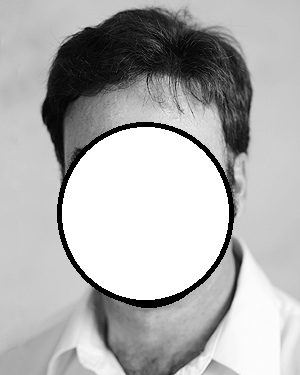
\includegraphics[width=1in,height=1.25in,clip,keepaspectratio]{author1.png}}]{First A. Author} received the B.S. and M.S. degrees in aerospace engineering from
the University of Virginia, Charlottesville, in 2001 and the Ph.D. degree in
mechanical engineering from Drexel University, Philadelphia, PA, in 2008.

From 2001 to 2004, he was a Research Assistant with the Princeton Plasma
Physics Laboratory. Since 2009, he has been an Assistant Professor with the
Mechanical Engineering Department, Texas A{\&}M University, College Station.
He is the author of three books, more than 150 articles, and more than 70
inventions. His research interests include high-pressure and high-density
nonthermal plasma discharge processes and applications, microscale plasma
discharges, discharges in liquids, spectroscopic diagnostics, plasma
propulsion, and innovation plasma applications. He is an Associate Editor of
the journal \emph{Earth, Moon, Planets}, and holds two patents.

Dr. Author was a recipient of the International Association of Geomagnetism
and Aeronomy Young Scientist Award for Excellence in 2008, and the IEEE
Electromagnetic Compatibility Society Best Symposium Paper Award in 2011.
\end{IEEEbiography}


\begin{IEEEbiography}[{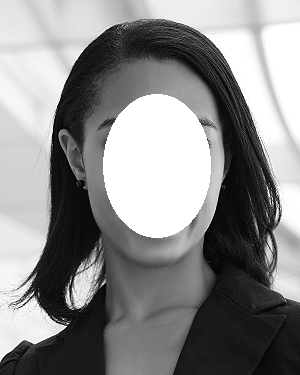
\includegraphics[width=1in,height=1.25in,clip,keepaspectratio]{author2.png}}]{Second B. Author} (M'76--SM'81--F'87) and all authors may include
biographies. Biographies are often not included in conference-related
papers. This author became a Member (M) of IEEE in 1976, a Senior
Member (SM) in 1981, and a Fellow (F) in 1987. The first paragraph may
contain a place and/or date of birth (list place, then date). Next,
the author's educational background is listed. The degrees should be
listed with type of degree in what field, which institution, city,
state, and country, and year the degree was earned. The author's major
field of study should be lower-cased.

The second paragraph uses the pronoun of the person (he or she) and not the
author's last name. It lists military and work experience, including summer
and fellowship jobs. Job titles are capitalized. The current job must have a
location; previous positions may be listed
without one. Information concerning previous publications may be included.
Try not to list more than three books or published articles. The format for
listing publishers of a book within the biography is: title of book
(publisher name, year) similar to a reference. Current and previous research
interests end the paragraph.

The third paragraph begins with the author's
title and last name (e.g., Dr.\ Smith, Prof.\ Jones, Mr.\ Kajor, Ms.\ Hunter).
List any memberships in professional societies other than the IEEE. Finally,
list any awards and work for IEEE committees and publications. If a
photograph is provided, it should be of good quality, and
professional-looking. Following are two examples of an author's biography.
\end{IEEEbiography}

\newpage

%If you do not have or do not want to include a photo, you can use IEEEbiographynophoto as shown below:

\begin{IEEEbiographynophoto}{Third C. Author, Jr.} (M'87) received the B.S. degree in mechanical
engineering from National Chung Cheng University, Chiayi, Taiwan, in 2004
and the M.S. degree in mechanical engineering from National Tsing Hua
University, Hsinchu, Taiwan, in 2006. He is currently pursuing the Ph.D.
degree in mechanical engineering at Texas A{\&}M University, College
Station, TX, USA.

From 2008 to 2009, he was a Research Assistant with the Institute of
Physics, Academia Sinica, Tapei, Taiwan. His research interest includes the
development of surface processing and biological/medical treatment
techniques using nonthermal atmospheric pressure plasmas, fundamental study
of plasma sources, and fabrication of micro- or nanostructured surfaces.

Mr. Author's awards and honors include the Frew Fellowship (Australian
Academy of Science), the I. I. Rabi Prize (APS), the European Frequency and
Time Forum Award, the Carl Zeiss Research Award, the William F. Meggers
Award and the Adolph Lomb Medal (OSA).
\end{IEEEbiographynophoto}

\EOD

\end{document}
